\documentclass[10pt]{article}
\usepackage[margin=0.5in]{geometry}
\usepackage{amsmath}
\usepackage{enumitem}
\usepackage{multicol}
\usepackage{tikz}
\usepackage{soul}

\newcommand{\ds}{\displaystyle}
\newcommand{\on}{\operatorname}


%%%%%%%%%%%%%%%%%%%%%%%%%%%%%%%%%%%%%%%%%%%%%%%%%%%%%%%%%%%%%%%%%%%%%%%%%%%%%%%%%%%%%%%%%%%%%%
%%% !!! NOTE FOR NEXT TIME !!!                                                             %%% 
%%% This homework was just a little too hard.  I'd simplify #4, #5, #7, and #11 next time. %%%
%%%%%%%%%%%%%%%%%%%%%%%%%%%%%%%%%%%%%%%%%%%%%%%%%%%%%%%%%%%%%%%%%%%%%%%%%%%%%%%%%%%%%%%%%%%%%%

\begin{document}
\newcounter{enumCount}
\pagestyle{empty}
\subsection*{Homework 7 - Math 140 \hfill Name: \underline{\hspace*{2in}}}

\noindent
\textit{Calculate the following derivatives.  }


\begin{multicols}{2}
\begin{enumerate}
\item $\ds \frac{d}{dx} 6 \sqrt{x}$
\item $\ds \frac{d}{dx} \frac{3}{x^2}$
\setcounter{enumCount}{\theenumi}
\end{enumerate}
\end{multicols}
\vfill

\begin{multicols}{2}
\begin{enumerate}
\setcounter{enumi}{\theenumCount}
\item $\ds \frac{d}{dt} 16t^2 - 64t + 100$
\item $\ds \frac{d}{dp} \left( p^{-2} - p^2 \right)$
\setcounter{enumCount}{\theenumi}
\end{enumerate}
\end{multicols}
\vfill

\begin{multicols}{2}
\begin{enumerate}
\setcounter{enumi}{\theenumCount}
\item $\ds \frac{d}{dt} 2t^3(t^2 + \sqrt{t})$
\item $\ds \frac{d}{dx} (x-5)(x+3)$
\setcounter{enumCount}{\theenumi}
\end{enumerate}
\end{multicols}
\vfill


\noindent
\textit{Find the slope of the tangent line for the following functions at the indicated point.}

\begin{multicols}{2}
\begin{enumerate}
\setcounter{enumi}{\theenumCount}
\item $\ds y= 4 - 3x - x^2$ at $x=1$.

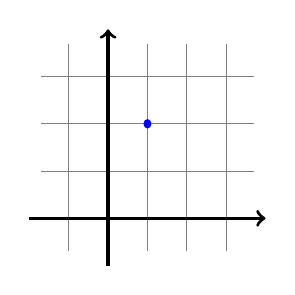
\begin{tikzpicture}[yscale=0.6,xscale=0.5]
\draw[gray] (-1.7,-0.7) grid (3.7,3.7);
\draw[very thick,->] (-2,0) -- (4,0);
\draw[very thick,->] (0,-1) -- (0,4);
\draw[very thick,color=blue] plot[domain=-1.2:2.2,samples=400] function {2+x-x**2};
\fill[blue,xscale=1] (1,2) circle (0.1);
\end{tikzpicture}

\item $\ds y = \frac{4}{x^2}$ at $x = -1$.

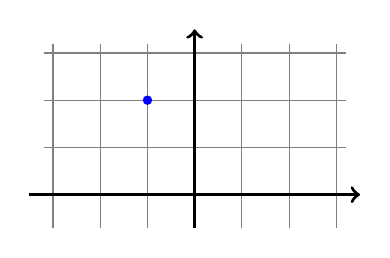
\begin{tikzpicture}[yscale=0.6,xscale=0.6]
\draw[gray] (-3.2,-0.7) grid (3.2,3.2);
\draw[very thick,->] (-3.5,0) -- (3.5,0);
\draw[very thick,->] (0,-0.7) -- (0,3.5);
\draw[very thick,color=blue] plot[domain=-3.2:-0.8,samples=400] function {2/(x**2)};
\draw[very thick,color=blue] plot[domain=0.8:3.2,samples=400] function {2/(x**2)};
\fill[blue,xscale=1] (-1,2) circle (0.1);
\end{tikzpicture}

\setcounter{enumCount}{\theenumi}
\end{enumerate}
\end{multicols}
\vspace*{0.75in}

\newpage
\noindent
\textit{Where do the following functions have horizontal tangent lines? Hint: find the derivatives first, then solve for when the derivative equals zero.}
\begin{multicols}{2}
\begin{enumerate}
\setcounter{enumi}{\theenumCount}

\item $\ds f(x) =  x^3-3x^2$ 

\item $\ds y= \tfrac{1}{5} x^{5} - \tfrac{7}{4} x^{4} + 4 x^{3}$. 
\setcounter{enumCount}{\theenumi}
\end{enumerate}
\end{multicols}
\vfill

\noindent
\textit{Solve the following.}
\begin{enumerate}
\setcounter{enumi}{\theenumCount}
\item A company estimates that if they hire $L$ workers, the output of their factor will be $Q(L) = 600 L^{2/3}$.  Find the derivative $Q'(x)$, then use $Q'(1000)$ to estimate how much output will increase if they have 1,000 workers and hire one more.
\vfill

\item A ball thrown in the air has a height of $h(t) = 6 + 29 t - 16t^2$ feet, where $t$ is time in seconds.  If the ball hits the ground at $t = 2$ seconds, calculate how fast the ball is falling then.  Recall that velocity is the derivative of the position (i.e., the height). 
\vfill

\end{enumerate}

\end{document}


%\item A fertilizer company estimates that if they produce $x$ tons of fertilizer, their revenue will be $R(x) = \dfrac{2x}{\left( 1+\frac{1}{200}x^2 \right)}$ (in thousands of dollars).  Find the marginal revenue $R'(10)$.  If the company is currently producing $10$ tons of fertilizer, should they increase or decrease production to increase revenue?
%\vfill
%
%
%\item Suppose 6 lbs. of salt is dissolved in a tank containing 50 gallons of water.  If the amount of water in the tank is increasing at 1 gallon per minute, then the concentration of the salt is $C(t) = \dfrac{6}{50+t}$ pounds per gallon.  What is the rate at which the concentration is decreasing after 10 minutes?
%\vfill
%
%
%\setcounter{enumCount}{\theenumi}
%\end{enumerate}
%
%
%\noindent
%In 2021, the Virginia state income tax for individuals is calculated as follows.
%\begin{center}
%\begin{tabular}{l|l}
%\hline
%Taxable Income & Tax Calculation \\ \hline
%0 to \$3,000 & 2\% \\
%\$3,000 to \$5,000  & \$60 $+$ 3\% of excess over \$3,000 \\
%\$5,000 to \$17,000 & \$120 $+$ 5\% of excess over \$5,000 \\
%\$17,000$+$  & \$720 $+$ 5.75\% of excess over \$17,000 \\ \hline
%\end{tabular} 
%\end{center}
%\begin{enumerate}
%\setcounter{enumi}{\theenumCount}
%\item The derivative of $T(x)$ is called the marginal tax rate.  Find the formula for $T(x)$ when $x$ is over \$17,000.  Then find the derivative $T'(x)$ for that tax bracket.  
%\vfill 
%
%\setcounter{enumCount}{\theenumi}
%\end{enumerate}


\end{document}
